\documentclass[10pt]{beamer}

%%%
% PREAMBLE FOR THIS DOC 
%%%
%https://tex.stackexchange.com/questions/68821/is-it-possible-to-create-a-latex-preamble-header
\usepackage{/Users/miw267/Repos/latex_preamble/beamer_preamble}



%%% TRY TO RESHOW TOC AT EACH SECTION START (with current section highlighted)
% Reference: https://tex.stackexchange.com/questions/280436/how-to-highlight-a-specific-section-in-beamer-toc
\newcommand\tocforsect[2]{%
  \begingroup
  \edef\safesection{\thesection}
  \setcounter{section}{#1}
  \tableofcontents[#2,currentsection]
  \setcounter{section}{\safesection}
  \endgroup
}


%%%% HERES HOW TO DO IT CORRECTLY
% FIRST IN .STY FILE, DO
%\usetheme[sectionpage=none]{metropolis}
% THEN AT EACH SECTION DO
%\begin{frame}{Outline}
%  \tableofcontents[currentsection]	
%\end{frame}



%\setbeamertemplate{navigation symbols}{}
%\setbeamertemplate{footline}[frame number]{}


%%%
% DOCUMENT
%%%

\begin{document}

%\maketitle

%% Title page frame
%\begin{frame}
%    \titlepage 
%\end{frame}





\title{10/14/2026: Induction}
\author{CSCI 246: Discrete Structures}
\date{Textbook reference: Scheinerman Sec. 22}

\begin{frame}
    \titlepage 
\end{frame}


\begin{frame}
\footnotesize 

\begin{mygreenbox}[title=Midterm Pickup]
Midterms are in the front of the room, grouped into four bins (A-G, H-L, M-R, S-Z) by last name. The midterms are upside down with your last name on the back. Come find yours before, during, or after class.  Only turn the quiz over if it's yours.
\end{mygreenbox} 
\vfill 
\begin{myredbox}[title=\text{Motivation: This course and the current job market}]
\begin{itemize}
\item \textbf{Mathematical reasoning is harder for AI to replace. } The work most exposed to automation is routine junior coding. Understanding why a model or algorithm behaves the way it does, judging whether an experiment is sound and reasoning about uncertainty are harder to automate. 
\item \textbf{Specialized roles are doing better than generalist ones}: For example, AI/ML engineering is up 39\% since 2022.
\end{itemize}
\end{myredbox}


\begin{myyellowbox}[title=Today's Agenda]
\begin{itemize}
	\item Quiz retake, midterm Review  ($\approx$ 5 mins)
	\item Mini-lecture ($\approx$ 25 mins)
	\item Group exercises ($\approx$ 20 mins)
\end{itemize}
\end{myyellowbox}
\vfill 

\end{frame}



\begin{frame}[standout]
Notes on Quiz Retake, Midterm
\end{frame}

\begin{frame}{Quiz Retake Results}

\begin{center}
You improved your scores by quite a bit! 
\includegraphics[width=0.1\textwidth]{images/high_five}
\end{center}
\vfill 

\begin{figure}
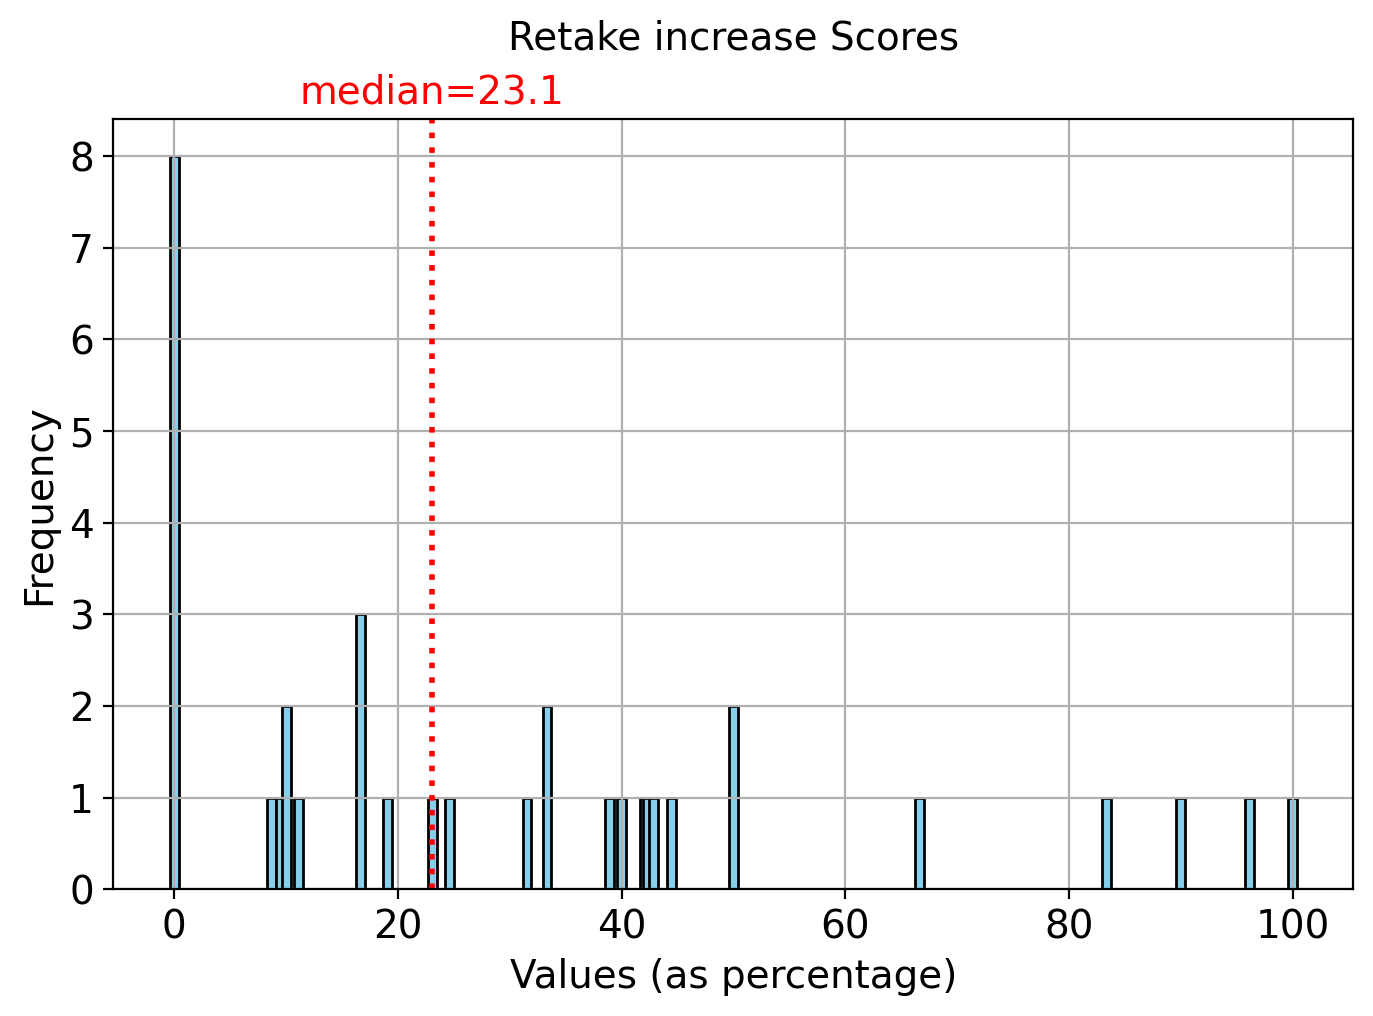
\includegraphics[width=.7\textwidth]{images/retake_increase_histogram.png}
\end{figure}
\vfill
\pause 
\begin{center}
\scriptsize (Apologies to those who had already maxed out their score.)
\end{center}
\end{frame}


\begin{frame}{Midterm Results}

\begin{figure}
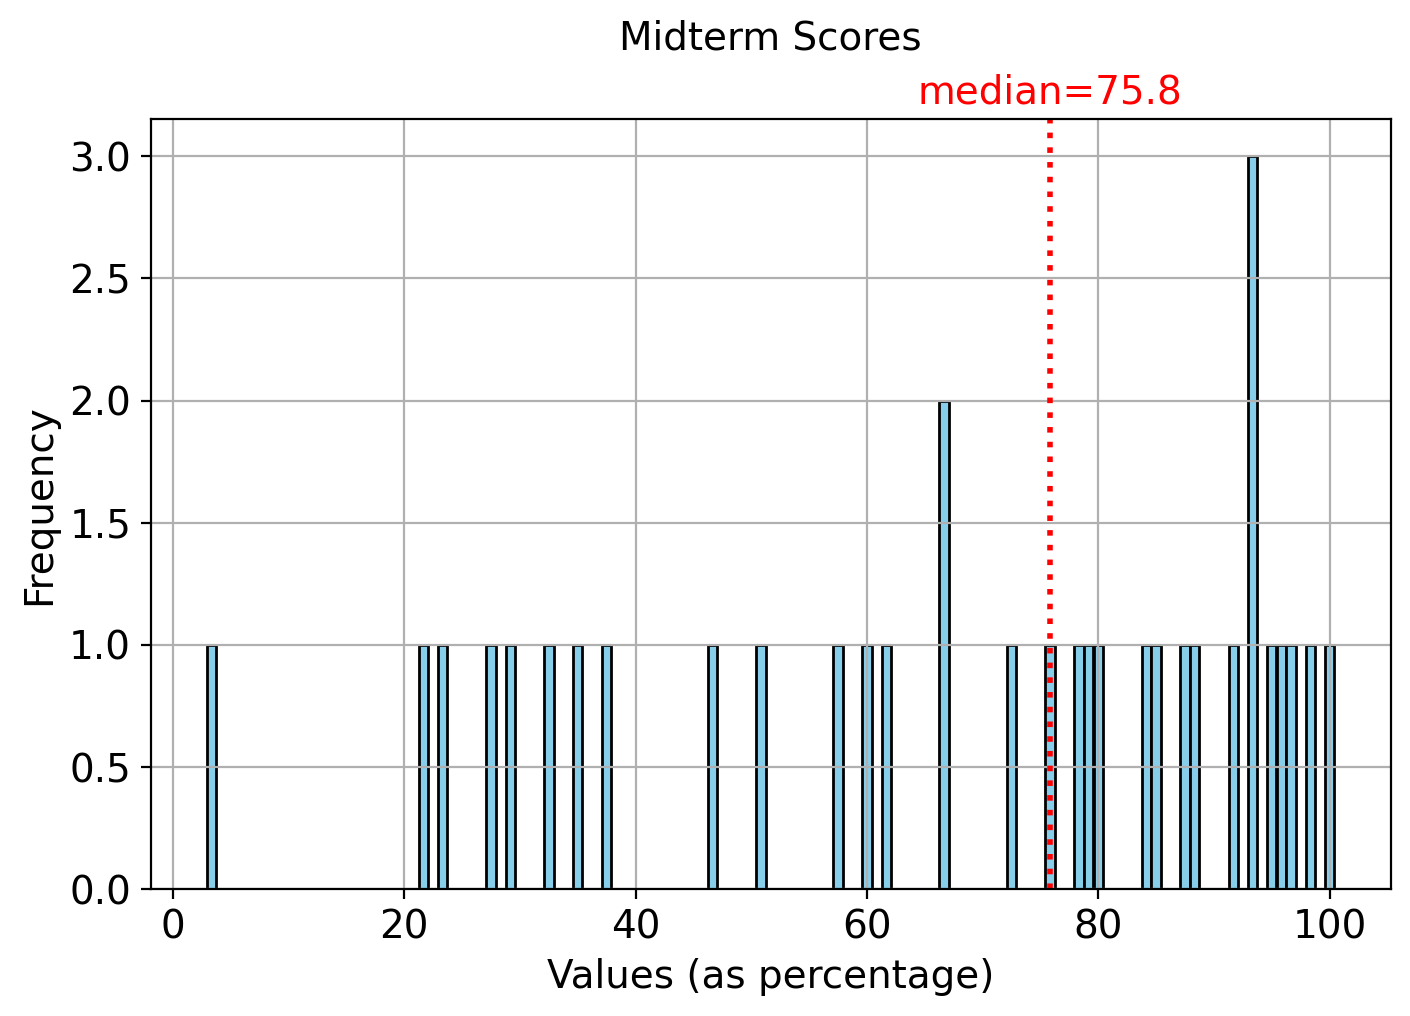
\includegraphics[width=.7\textwidth]{images/midterm_histogram.png}
\end{figure}
%\vfill
%\pause 
%\begin{center}
%\scriptsize (Apologies to those who had already maxed out their score.)
%\end{center}
\end{frame}


\begin{frame}{What you could do if your midterm score is lower than you'd like?}

Consider rethinking your preparation strategy...

\begin{enumerate}
	\item<1-> Are you \alert{(actively)} reading the textbook before class? 
	\item<2-> Are you attending class?
	\only<2>{
	\begin{figure}
	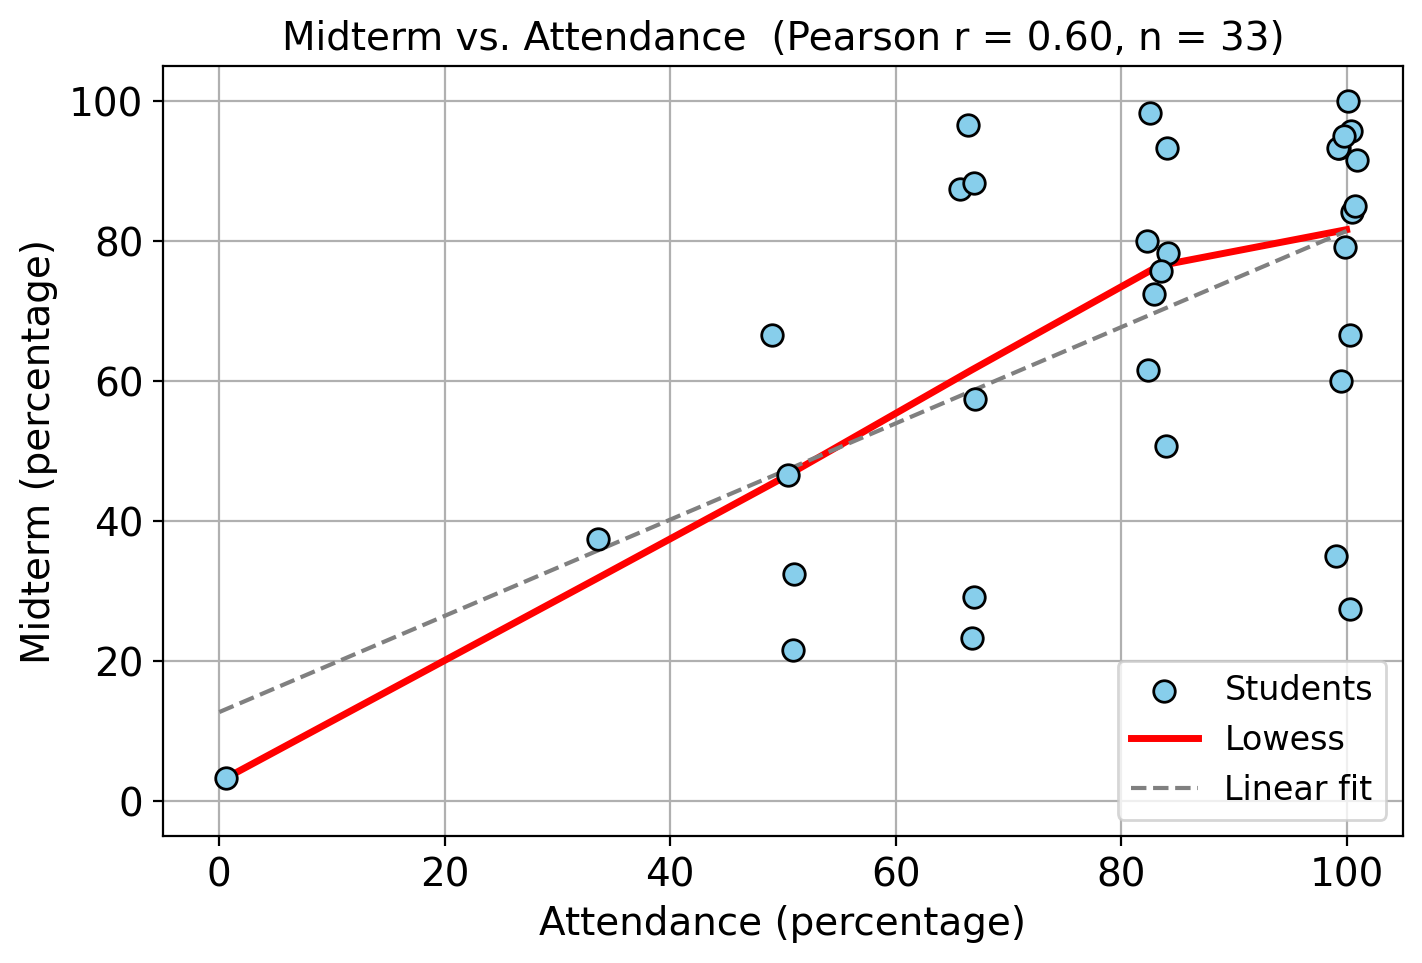
\includegraphics[width=.7\textwidth]{images/midterm_vs_attendance.png}
	\end{figure}
	}
	\item<3-> Are you finishing the group exercises after class?
	\item<4-> Take advantage of office/tutoring hours.
	\item<5-> Come chat with me to brainstorm on the details.
\end{enumerate}


\vfill 

\only<6->{
\colorbox{green!30}{\textbf{Opportunity.}} I will offer optional midterm retakes.  Details forthcoming.
}
%\vfill
%\pause 
%\begin{center}
%\scriptsize (Apologies to those who had already maxed out their score.)
%\end{center}
\end{frame}


\begin{frame}[standout]
Study Guide for Quiz 6
\end{frame}


\begin{frame}{Study Guide For Quiz 6}
\footnotesize 

\colorbox{yellow!20}{\textbf{Group exercises.}} Know how to solve the group exercises from the course meetings on Binomial Coefficients (9/26) and Contradiction and Contraposition (10/3).  


\vfill 

\colorbox{red!20}{\textbf{Readings.}}  \\
\vspace{.2cm}
Sec. 17 (Binomial Coefficients )
\begin{itemize}
\item Understand Def 17.1, as used in Examples 17.2-17.4 and 17.6.
\item Understand how to apply the computational formula of Theorem 17.12.
\item Understand the intuition behind Prop 17.7.
\end{itemize}
Sec. 20 (Contradiction and Contraposition)
\begin{itemize}
\item Understand how to apply Proof Template 11.
\item Understand how to apply Proof Template 12, as used to prove Proposition 20.3.
\end{itemize}

\vfill 
\pause 
\colorbox{green!20}{\textbf{Extra credit proof review question.}}  I will give 10\% extra credit on your midterm if you can answer the review question \underline{perfectly.}  

\begin{center}
\textit{Let $x$ be an integer. Prove that $0 \mid x$ if and only if $x=0$.} 
\end{center}
For a solution, see Group Exercise \#3 from the  slide deck on proofs (09/02/26).
\end{frame}


\begin{frame}[standout]
Induction
\end{frame}


\begin{frame}{Induction Demo}


\begin{center}
\colorbox{green!30}{\textbf{Good news!}} I'm going to \alert{pay} you to learn induction! 
\includegraphics[width=0.2\textwidth]{images/money}
\end{center}
\vfill 
\pause 

\colorbox{yellow!30}{\textbf{Rule.}}
\begin{itemize}
\item \textbf{(Base)} Student $n=1$ gets a coin.
\item \textbf{(Step)} If student $n-1$ gets a coin, then student $n$ gets a coin.
\end{itemize}

\vfill
\pause

\colorbox{blue!30}{\textbf{Results.}}
\begin{center}
\begin{tabular}{c c l}
\toprule
\textbf{Student ID} & \textbf{Gets a coin?} & \textbf{Reason} \\
\midrule
\pause
1 & Yes & Base \\
\pause
2 & Yes & Step applied to student 1 \\
\pause
3 & Yes & Step applied to student 2 \\
\pause
4 & Yes & Step applied to student 3 \\
\pause 
\vdots & \vdots & \vdots \\
\bottomrule
\end{tabular}
\end{center}

\vfill
\end{frame}


\begin{frame}{Triangular Numbers}



% \begin{mygreenbox}[title=Triangular Numbers]
%Last class, we showed that the $n$-th triangular number is $n(n+1)/2$.  That is, we proved 
%\[1+ 2+ 3+ \cdots + n = n(n+1)/2.\]
%\begin{figure}[ht]
% \centering
% 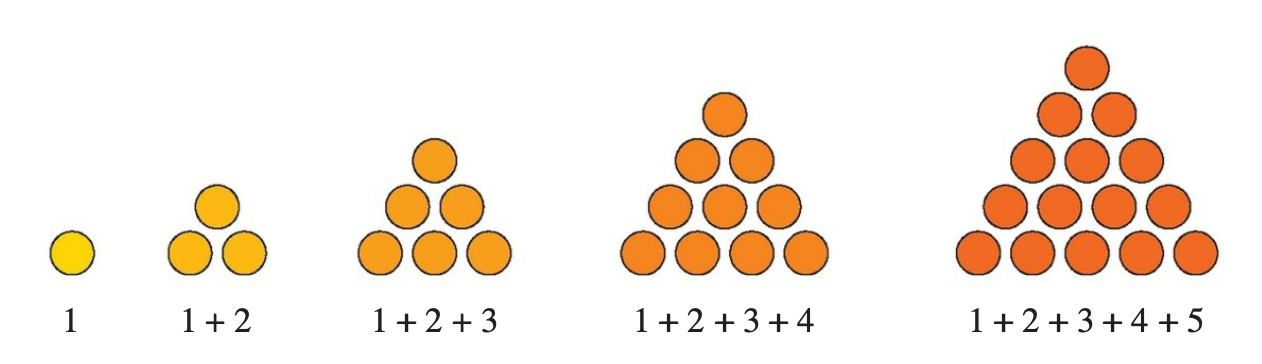
\includegraphics[width=0.6\textwidth]{images/triangular_numbers}
%\end{figure}
%\end{mygreenbox}


 \begin{myyellowbox}[title=Poll]
 Last class, we proved 
 \[1+ 2+ 3+ \cdots + n = n(n+1)/2.\]
What is the intuition behind this formula?
\end{myyellowbox}


\vfill 
\pause 


 \begin{mygreenbox}[title=Hint]
\begin{figure}[ht]
 \centering
 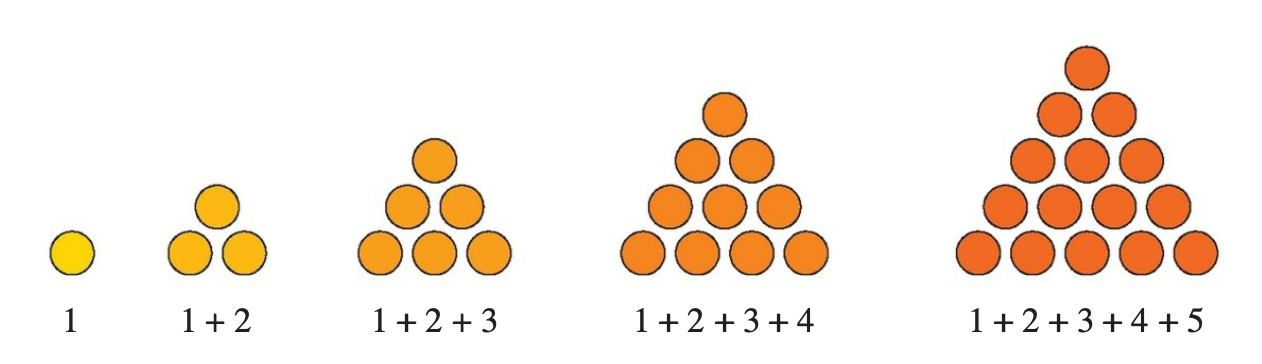
\includegraphics[width=0.6\textwidth]{images/triangular_numbers}
\end{figure}
\end{mygreenbox}


\end{frame}






\begin{frame}{Triangular Numbers: Geometric Intuition}
\small 
%Here's a case where \textbf{geometry makes the algebra obvious}.
\vfill 
\begin{mybluebox}[title=Triangular Numbers]
\begin{center}
The $n$-th triangular number is

\[T_n = 1 + 2 + 3 + \dots + n = \frac{n(n+1)}{2}. \]

It counts the number of dots you can arrange in an \textbf{triangle} like this:

\vspace{.5cm}
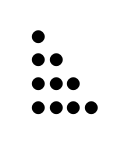
\begin{tikzpicture}[scale=0.3, every node/.style={inner sep=1pt}]
% Right triangle (flipped horizontally)
\foreach \i in {1,...,4}{
  \foreach \j in {1,...,\i}{
    \node at (5 + 0.75*\i - 0.75*\j, -\i) {\large $\bullet$};
  }
}
\end{tikzpicture}
\vspace{.5cm}
%for $T_4$.
\end{center}
\end{mybluebox}

\end{frame}

%
%\begin{frame}{Triangular Numbers: Geometric Intuition}
%\begin{mygreenbox}[title=\text{Geometric Intuition: Make a rectangle from two triangles}]
%
%If you put together \textbf{two copies} of that triangle, it forms a \textbf{rectangle}.
%
%\begin{center}
%\begin{tikzpicture}[scale=0.3, every node/.style={inner sep=1pt}]
%
%% Left triangle
%\foreach \i in {1,...,4}{
%  \foreach \j in {1,...,\i}{
%    \node at (0.75*\j - 0.75*\i, -\i) {\large $\bullet$};
%  }
%}
%
%
%% Right triangle (flipped horizontally)
%\foreach \i in {1,...,4}{
%  \foreach \j in {1,...,\i}{
%    \node at (5 + 0.75*\i - 0.75*\j, -\i) {\large $\bullet$};
%  }
%}
%
%% Plus sign between them
%\node[scale=2] at (2.3, -2) {$+$};
%
%% Optional: show rectangle outline (comment out if you want just dots)
%%\draw[gray, dashed, thick] (-1.2, -4.6) rectangle (6.2, -0.4);
%
%\end{tikzpicture}
%\end{center}
%
%If you flip one triangle and fit it next to the other, you get a rectangle with:
%
%\begin{itemize}
%\item \textbf{Height:} $n$ dots
%\item \textbf{Width:} $n+1$ dots
%\end{itemize}
%
%So the rectangle has \textbf{area} $n(n+1)$ dots. \\
%
%But that rectangle is made of \textbf{two identical triangles}, so the number of dots in each triangle is
%
%\[T_n = \frac{n(n+1)}{2}.\]
%
%\end{mygreenbox}
%
%\end{frame}


\begin{frame}{Triangular Numbers: Geometric Intuition}
\small
\begin{mygreenbox}[title=\text{Geometric Intuition: Make a rectangle from two triangles}]

Take \textbf{two copies} of the triangle for $T_4$. \only<2->{Rotate one copy by $180^\circ$.} \only<3->{Then slide it into place: the two triangles fit together into a \textbf{rectangle}.}

\begin{center}
\begin{tikzpicture}[scale=0.42, dot/.style={circle, inner sep=0pt, minimum size=5pt}]
\path[use as bounding box] (-0.5,0) rectangle (12.5,-5.9);

% Blue triangle: row i has i dots (always shown, never moves)
\foreach \i in {1,...,4}{
  \foreach \j in {1,...,\i}{
    \node[dot, fill=blue] at (\j,-\i) {};
  }
}

% Step 1: an identical red copy
\only<1>{
  \node at (6.5,-2.5) {\Large $+$};
  \foreach \i in {1,...,4}{
    \foreach \j in {1,...,\i}{
      \node[dot, fill=red] at (7+\j,-\i) {};
    }
  }
}

% Step 2: the red copy rotated 180 degrees (row i now has 5-i dots)
\only<2>{
  \node at (6.5,-2.5) {\Large $+$};
  \foreach \i in {1,...,4}{
    \foreach \j in {\i,...,4}{
      \node[dot, fill=red] at (7+\j,-\i) {};
    }
  }
  \node[red, font=\scriptsize] at (10,-5.2) {rotated $180^\circ$};
}

% Step 3: red copy slid next to the blue one, filling each row out to 5 dots
\only<3->{
  \foreach \i in {1,...,4}{
    \pgfmathtruncatemacro{\start}{\i+1}
    \foreach \j in {\start,...,5}{
      \node[dot, fill=red] at (\j,-\i) {};
    }
  }
  \draw[gray, dashed] (0.5,-0.5) rectangle (5.5,-4.5);
  \draw[decorate, decoration={brace, mirror, amplitude=4pt}] (0.5,-4.8) -- (5.5,-4.8)
    node[midway, below=4pt, font=\scriptsize] {width $n+1 = 5$};
  \draw[decorate, decoration={brace, amplitude=4pt}] (5.8,-0.5) -- (5.8,-4.5)
    node[midway, right=5pt, font=\scriptsize] {height $n = 4$};
}
\end{tikzpicture}
\end{center}

\uncover<4->{
So the rectangle has \textbf{area} $n(n+1)$ dots.  But it is made of \textbf{two identical triangles}, so the number of dots in each triangle is
\[T_n = \frac{n(n+1)}{2}.\]
}

\end{mygreenbox}
\end{frame}




\begin{frame}{The Induction Strategy to Proving Things}
\small
 \begin{mygreenbox}[title=Problem]
Prove that the $n$-th triangular number is $n(n+1)/2$.  That is, prove 
%
\begin{align*}
1+ 2+ 3+ \cdots + n = n(n+1)/2.
\end{align*}
%
\end{mygreenbox}

\vfill 

 \begin{myyellowbox}[title=Induction Strategy]
\begin{figure}
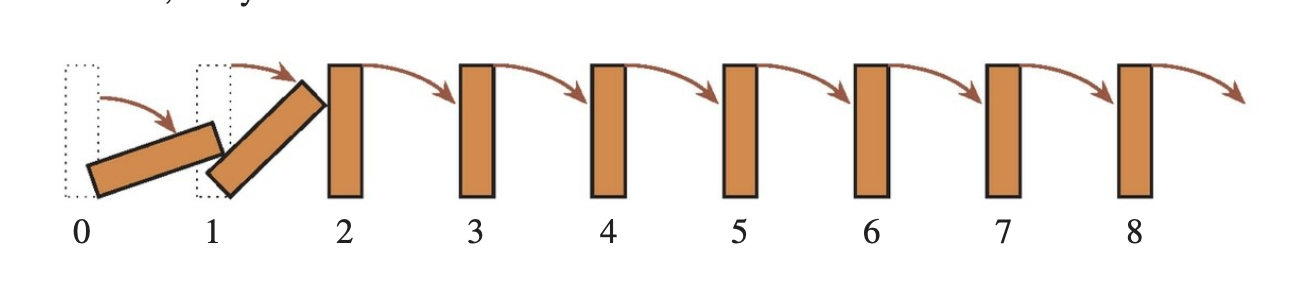
\includegraphics[width=\textwidth]{images/dominos.png}
\end{figure}

\textbf{Base.} Show the equation holds for some starting point (usually 0 or 1).

\textbf{Induction step.} Show that if the equation holds for natural number $n=k$, then it must hold for natural number $n=k+1$.   
 \end{myyellowbox}

\vfill 
The strategy in the \gold{yellow box} lets us conclude the equation holds for all $n$.
\end{frame} 



\begin{frame}{Proof By Induction: Example}
\small
 \begin{mygreenbox}[title=Problem (Induction)]
Prove that the $n$-th triangular number is $n(n+1)/2$.  That is, prove 
%
\begin{equation}
\bluemathbox{1+ 2+ 3+ \cdots + n} = \bluemathbox{\frac{n(n+1)}{2}}.
\label{eqn:triangular_number_identity}
\end{equation}
\vspace{-0.6cm}
\end{mygreenbox}
\vspace{-0.3cm}
\textbf{Base.} We show \Eqref{eqn:triangular_number_identity} holds for $n=1$.  In that case, \Eqref{eqn:triangular_number_identity} says
\[ 1 = \frac{1(1+1)}{2}  \]
which is true. \\

\pause 
\textbf{Induction step.}  We assume \Eqref{eqn:triangular_number_identity} holds for $n=k$, where $k\geq 1$, which was the base case. (This is called the \alert{induction hypothesis}.)  We show \Eqref{eqn:triangular_number_identity} holds for $n=k+1$.  That is, we must show
 %
 \begin{equation}
\bluemathbox{1+ 2+ 3+ \cdots + k} + \redmathbox{(k+1)} = \frac{(k+1)(k+2)}{2}.
\label{eqn:triangular_number_inductio_step}
\end{equation}
%
\vspace{-.1cm}
\pause We have
%
\begin{align*}
 \text{LHS of \Eqref{eqn:triangular_number_inductio_step}} &= \bluemathbox{\frac{k(k+1)}{2}} \; + \; \redmathbox{(k+1)} && \scripttext{(by induction hypothesis)}\\
 &=  \text{RHS of \Eqref{eqn:triangular_number_inductio_step}} && \scripttext{(after some algebra)}	
\end{align*}
\end{frame}


\begin{frame}{Induction and Strong Induction}
\footnotesize
What we've been using so far is \alert{classical} induction.

 \begin{mygreenbox}[title=\text{Scheinerman Theorem 22.2: Induction}]
Let $A$ be a set of natural numbers. If
\begin{itemize}
	\item $0 \in A$, and 
	\only<1-2>{\item $\forall k \in \mathbb{N}, k \in A \implies k+1 \in A$}
	\only<3->{	\item $\forall k \in \mathbb{N}, \alert{k \in A} \implies k+1 \in A$}
\end{itemize}
then $A=\mathbb{N}$.
\end{mygreenbox}

\vfill
\pause 	

There is also a \alert{strong} version.

 \begin{mygreenbox}[title=\text{Scheinerman Theorem 22.9: Strong Induction}]
Let $A$ be a set of natural numbers. If
\begin{itemize}
	\item $0 \in A$, and 
	\only<2>{\item $\forall k \in \mathbb{N}, \; \set{0,1,2,\cdots, k} \subset A \implies k+1 \in A$}
	\only<3->{\item $\forall k \in \mathbb{N}, \; \alert{\set{0,1,2,\cdots, k} \subset A} \implies k+1 \in A$}
\end{itemize}
then $A=\mathbb{N}$.
\end{mygreenbox}
\pause 
\colorbox{blue!30}{\textbf{Remark.}} If the result you wish to prove doesn't cover all natural numbers -- say it covers just the positive integers -- the basis step may begin at a value other than 0.
\end{frame}


\begin{frame}{Strong Induction}
%\footnotesize
% \begin{mygreenbox}[title=Strong Induction]
%Assume that $A$ is a set of natural numbers with the property that, for every natural number $n$, if every number smaller than $n$ is in $A$, then $n$ itself is in $A$. Then every natural number is in $A$.
%\end{mygreenbox}
%
%\vfill 

 \begin{myredbox}[title=When to Use Strong Induction]
 Sometimes there are scenarios where the induction implication goes naturally not from $n$ to $n+1$, but:
 \begin{itemize}
 \item From some smaller number to $n+1$, or
 \item From several smaller numbers	
 \end{itemize}
 \end{myredbox}

\vfill 
\pause 
 \begin{myyellowbox}[title=Example: Every positive integer has a prime factorization]
 \begin{itemize}
 \item Suppose every number smaller than $n$ has a prime factorization.
 \item The number $n$ must either be prime (in which case we are done) or composite.
 \item If $n$ is composite, then $n=ab$ for smaller number $a,b<n$.  But $a,b$ have their own  factorizations by the induction hypothesis.  These can be put together to make a prime factorization of $n$.
 \end{itemize}

 \end{myyellowbox}
\end{frame}


\begin{frame}[fragile]{Uses of induction in computer science: Examples}
\small 
\begin{enumerate}
	\item \textbf{Proving correctness of recursive algorithms:} E.g. we can use induction to show $\texttt{factorial}(n)=n!$.
%\resizebox{0.8\textwidth}{!}{%
\begin{python}
def factorial(n):
    """Compute n! recursively"""
    if n == 0:
        return 1
    else:
        return n * factorial(n - 1)
\end{python}
%}
\pause 
\item \textbf{Analyzing algorithm complexity:} To determine the complexity -- e.g. $\mathcal{O}(n \log n)$ -- of recursive algorithms (like mergesort, quicksort, binary search),  we often use induction on  $n$.
\pause 
\item \textbf{Proving properties of data structures:} Many structures (like linked lists, binary trees, heaps, etc.) are defined inductively.
%\pause 
%\item \textbf{Proving correctness of loops}: You show that some property holds before the loop. Then show if it holds at one iteration, it still holds at the next. 
\end{enumerate}
\end{frame}



\begin{frame}[standout]
Group exercises
\end{frame}


\begin{frame}{Random group assignments}
\begin{columns}
\begin{column}{0.33\textwidth}
Ashley, Isabelle: 3 \\ 
Bailey, Tanna: 13 \\ 
Blaisdell, Olyver: 13 \\ 
Brown, Ashton: 5 \\ 
Brown, Jonathan: 1 \\ 
Cardenas, Dominic: 11 \\ 
Cutler, George: 9 \\ 
Fabik, Roland: 3 \\ 
Fellows, Audrey: 8 \\ 
Fitzgerald, Ryan: 5 \\ 
Fuller, Ryan: 6 \\ 
Griffen, Clara: 10 \\ 
Grutsch, Tanner: 9 \\\end{column}
\begin{column}{0.33\textwidth}
Hager, Nathan: 7 \\ 
Horner, Jayden: 12 \\ 
Johnson, Jaret: 2 \\ 
Kintzel, Samantha: 4 \\ 
Lameres, Alexis: 4 \\ 
Lee, Holden: 1 \\ 
Mayala, Reece: 5 \\ 
McLean, Connor: 7 \\ 
Mcbride, Daniel: 3 \\ 
Miller, Maverick: 10 \\ 
Moss, Emily: 6 \\ 
Mousseau, Matthew: 12 \\\end{column}
\begin{column}{0.33\textwidth}
Neuman, Evan: 7 \\ 
Putnam, John: 2 \\ 
Ramos, Vydel: 8 \\ 
Rathbun, Jedidiah: 11 \\ 
Roberts, Matthew: 10 \\ 
Roller, Nathan: 1 \\ 
Ryan, Otis: 11 \\ 
Shevtsov, Timothy: 4 \\ 
Sinclair, Aidan: 8 \\ 
Stensland, Emma: 2 \\ 
Thiessen, Logan: 9 \\ 
Thompson, Jaiden: 6 \\ 
Vath, Ethan: 12 \\\end{column}
\end{columns}
\end{frame}








\begin{frame}{Group exercises: Induction}

\begin{enumerate}
\item Show by induction that $n^2-n$ is even for any natural number $n$ (that is, for $n=0,1,2,\hdots$).
\item  Show by induction that $2^n < n!$ for all $n \geq 4$.	
\item Show by induction that $f_0 + \cdots + f_n = f_{n+2} -1$ in the Fibonacci sequence.
\item Show by induction that $f_n < 2^n$ in the Fibonacci sequence. 
\end{enumerate}
\vfill 
\begin{mygreenbox}[title=Definition]
The \textbf{Fibonacci sequence} is the sequence given by the following recursive rules:
\[f_0 =0, \qquad \quad f_1 =1, \qquad \quad f_{n+2} = f_n + f_{n+1} \]
The sequence is: $0,1,1,2,3,5,8,13,21,34, \hdots$
\end{mygreenbox}


\end{frame}

\begin{frame}[standout]
Solutions to group exercises	
\end{frame}


\begin{frame}
\small 
\begin{mygreenbox}[title=Exercise 1]
Show by induction that $n^2-n$ is even for any natural number $n$ (that is, for $n=0,1,2,\hdots$).
\end{mygreenbox}

\vfill \vfill 
\begin{myyellowbox}[title=Solution (by Induction)]
\textbf{Induction base.} Take $n=0$.  Then $n^2-n = 0^2-0 = 0$, which is even. So $n^2-n$ is even when $n=0$.

\vspace{0.5cm}

\textbf{Induction step.} Now we \underline{assume} the proposition holds at index $k$ (this is called the \alert{induction hypothesis}), and we \underline{need to show} it holds at index $k+1$.  That is, we assume $k^2-k$ is even, and we need to show that $(k+1)^2-(k+1)$ is even.  We have
%
\begin{align*}
(k+1)^2-(k+1) &= (k^2+2k+1) - (k+1) \\
&= k^2+k  \\
&= \explaintermbrace{even by induct. hypoth.}{(k^2 -k)} \; + \; \explaintermbrace{even by def. even}{(2k)}  && \scripttext{(subtract, add $n$)}	
\end{align*}
And the sum of two even numbers is even.

Hence, $k^2-k$ is even $\implies (k+1)^2-(k+1)$ is even.
\end{myyellowbox}

\end{frame}

\begin{frame}
\begin{mygreenbox}[title=Exercise 2]
 Show by induction that $2^n < n!$ for all $n \geq 4$.	
\end{mygreenbox}

\vfill \vfill 
\begin{myyellowbox}[title=Solution]
\textbf{Induction base.} Take $n=4$.  Then $2^n = 2^4 = 16$ and $n! = 4! = 4 \cdot 3 \cdot 2 \cdot 1 = 24$. So $2^n < n!$ when $n=4$.

\vspace{0.5cm}

\textbf{Induction step.} Now we \underline{assume} the proposition holds at index $k$ (this is called the \alert{induction hypothesis}), and we \underline{need to show} it holds at index $k+1$.  That is, we \underline{assume} $2^k<k!$ (this is called the \alert{induction hypothesis}), and we \underline{need to show} $2^{k+1}<(k+1)!$ We have
%
\begin{align*}
2^{k+1} &= 2 \cdot 2^k \\
&< 2 \cdot k! && \scripttext{(by the induction hypothesis)} \\
&< (k+1) \cdot k! && \scripttext{(since $k \geq 4$)} \\
&= (k+1)! && \scripttext{(by def. factorial)}	
\end{align*}
Hence, $2^k<k! \implies 2^{k+1}<(k+1)!$
\end{myyellowbox}
\end{frame}




\begin{frame}

\begin{mygreenbox}[title=Exercise 3]
Show by induction that $f_0 + \cdots + f_n = f_{n+2} -1$ in the Fibonacci sequence.	
\end{mygreenbox}

\vfill \vfill 
\begin{myyellowbox}[title=Solution]
\textbf{Induction base.} Take $n=0$.  Then $f_0 + \cdots + f_n = f_0 =0$ and $f_{n+2} -1 = f_2 -1 = 1-1 = 0$. So $f_0 + \cdots + f_n = f_{n+2} -1$ when $n=0$.

\vspace{0.25cm}

\textbf{Induction step.} Now we \underline{assume} the proposition holds at index $k$ (this is called the \alert{induction hypothesis}), and we \underline{need to show} it holds at index $k+1$.  That is, we assume $f_0 + \cdots + f_k = f_{k+2} -1$, and we need to show that $f_0 + \cdots + f_{k+1} = f_{k+3} -1$.  We have
%
\begin{align*}
f_0 + \cdots + f_{k+1} &= (f_0 + \cdots + f_k) + f_{k+1} \\
&=(f_{k+2} -1) + f_{k+1} && \scripttext{(by the induction hypothesis)} \\
&= (f_{k+1}+f_{k+2}) -1  && \\
&= f_{k+3} -1  && \scripttext{(by def. Fibonacci number)}	
\end{align*}
Hence, if the proposition holds at index $k$, it holds at index $k+1$.
\end{myyellowbox}
	
\end{frame}


\begin{frame}
\small 
\begin{mygreenbox}[title=Exercise 4]
Show by induction that $f_n < 2^n$ in the Fibonacci sequence. 
\end{mygreenbox}

\vfill \vfill 
\begin{myyellowbox}[title=Solution]
\textbf{Induction base.} Take $n=0$.  Then $f_n = f_0 = 0$  and  $2^n =2^0 =1$. So $f_n < 2^n$ when $n=0$.

\vspace{0.25cm}

\textbf{Induction step.} Here we use strong induction. We \underline{assume} the proposition holds at indices $1, 2, \hdots k$ (this is the \alert{(strong) induction hypothesis}), and we \underline{need to show} it holds at index $k+1$.  That is, we assume $f_j < 2^j$ for $j=1,\hdots, k$, and we need to show that $f_{k+1} < 2^{k+1}$.  We have
%
\begin{align*}
f_{k+1} &= f_k + f_{k-1} && \scripttext{(by def. Fibonacci number)}	\\
&< 2^k + 2^{k-1} && \scripttext{(by the (strong) induction hypothesis)} \\
&< 2^k + 2^k  && \\
&= 2 \cdot 2^k  \\
&= 2^{k+1}.
\end{align*}
Hence, $f_k < 2^k \implies f_{k+1} < 2^{k+1}$.
\end{myyellowbox}
	
\end{frame}

\end{document}
